\section{Results}
%%%%%%%%%%%%%%%%%%%%%%%%%%%%%%%%%%%%%%%%%%%%%%%%%%%%%%%%%%%%%%%%%%%%%%
\label{sec:Results}

In order to unfold the spectrum, the procedure described in section \ref{sec:Unfolding} has been pursued.
The statistical plus type A systematic uncertainties are propagated by the unfolding procedure into the final spectrum, taking into account the signal strengths covariance matrix. The type B systematic uncertainty has been propagated using the following procedure: for each \pth bin, we compute the upper bound of the systematic band computing the square sum of all the signal strength variations that deviate in the up direction with respect to the bin central value, whether or not this variation corresponds to the up or down shift of the systematic uncertainty. The same is done for the lower bound of the systematic band. If both the up and down shifts of a given nuisance parameter lead to a same direction variation of the signal strength, only the larger variation is considered.

The unfolded \pth{} spectrum is shown in Fig.~\ref{fig:unfolded}. Statistical, systematic, and theoretical uncertainties are shown as separate error bands in the plot.
\begin{figure}[!h]
\centering
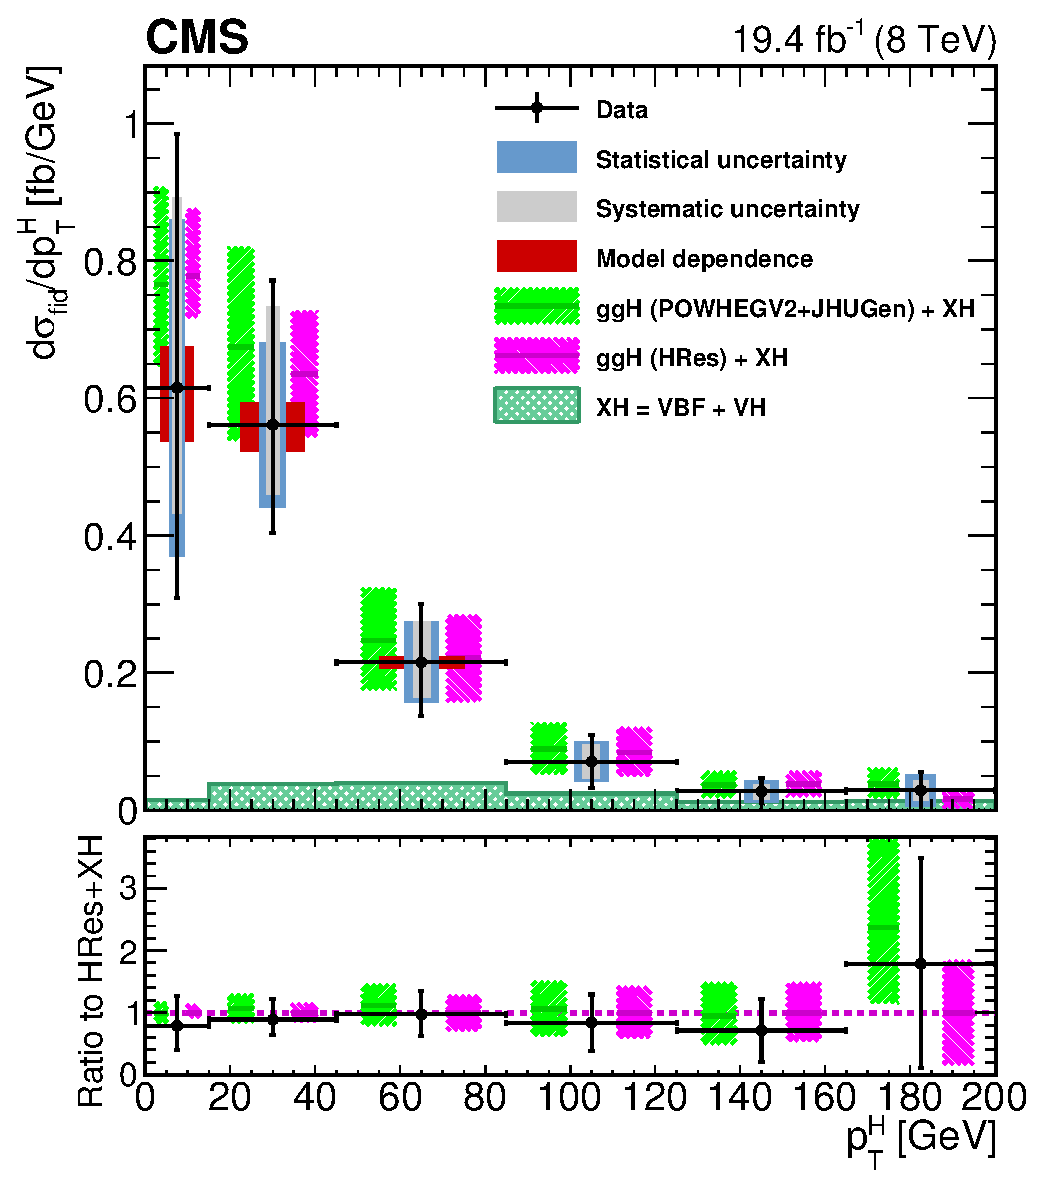
\includegraphics[width=0.8\textwidth]{images/unblinding/pthRatio_unfolded_paper.pdf}
\caption{Higgs boson production cross section as a function of \pth{}, after applying the unfolding procedure.
Data points are shown, together with statistical and systematic uncertainties. The vertical bars on the data points correspond to the sum in quadrature of the statistical and systematic uncertainties. The model dependence uncertainty is also shown.
The pink (and back-slashed filling) and green (and slashed filling) lines and areas represent the SM theoretical estimates in which the acceptance of the dominant ggH contribution is modelled by \textsc{HRes} and \textsc{Powheg V2}, respectively. The subdominant component of the signal is denoted as XH=VBF+VH and it is shown with the cross filled area separately. The bottom panel shows the ratio of data and \textsc{Powheg V2} theoretical estimate to the \textsc{HRes} theoretical prediction.}\label{fig:unfolded}
\end{figure}
The unfolded spectrum is compared with the SM-based theoretical predictions where the ggH contribution is modelled using the \textsc{HRes} and \textsc{Powheg V2} programs. The comparison shows good agreement between data and theoretical predictions within the uncertainties.
The measured values for the differential cross section in each bin of $p_{\rm T}^{\rm H}$ are reported together with the total uncertainty in Table~\ref{table:values_and_uncertainties}.

\begin{table}
\caption{Differential cross section in each \pth{} bin, together with the total uncertainty and the separate components of the various sources of uncertainty.}\label{table:values_and_uncertainties}
\footnotesize{
\begin{tabular}{ccccccc}
\hline\hline
\begin{tabular}[c]{@{}c@{}}\pth{}\\$\left[\mathrm{GeV}\right]$\end{tabular} & \begin{tabular}[c]{@{}c@{}}$d\sigma/dp_{\rm{T}}^{\rm H}$\\$\left[\mathrm{fb/GeV}\right]$\end{tabular} & \begin{tabular}[c]{@{}c@{}}Total uncertainty\\$\left[\mathrm{fb/GeV}\right]$\end{tabular} & \begin{tabular}[c]{@{}c@{}}Statistical\\uncertainty\\$\left[\mathrm{fb/GeV}\right]$\end{tabular} & \begin{tabular}[c]{@{}c@{}}Type A\\uncertainty\\$\left[\mathrm{fb/GeV}\right]$\end{tabular}& \begin{tabular}[c]{@{}c@{}}Type B uncertainty\\$\left[\mathrm{fb/GeV}\right]$\end{tabular} & \begin{tabular}[c]{@{}c@{}}Type C uncertainty\\$\left[\mathrm{fb/GeV}\right]$\end{tabular} \\ 
\hline
0-15 & 0.615 & +0.370/-0.307 & $\pm$0.246 & $\pm$0.179 & +0.211/-0.038  & +0.0782/-0.0608 \\ 
15-45 & 0.561 & +0.210/-0.157 & $\pm$0.120 & $\pm$0.093 & +0.146/-0.041  & +0.0395/-0.0327 \\ 
45-85 & 0.215 & +0.084/-0.078 & $\pm$0.059 & $\pm$0.037 & +0.047/-0.034  & +0.0089/-0.0084 \\ 
85-125 & 0.071 & +0.038/-0.038 & $\pm$0.029 & $\pm$0.017 & +0.018/-0.017  & +0.0018/-0.0022 \\ 
125-165 & 0.027 & +0.020/-0.019 & $\pm$0.016 & $\pm$0.009 & +0.007/-0.007  & +0.0003/-0.0006 \\ 
165-$\infty$ & 0.028 & +0.027/-0.027 & $\pm$0.023 & $\pm$0.012 & +0.008/-0.007  & +0.0002/-0.0006 \\ 
\hline 
\end{tabular}
}
\end{table}

Figure \ref{fig:cov_matrix} shows  the correlation matrix for the six bins of the differential spectrum. The correlation of of bins is defined as in Eq.~\eqref{eq:correlation}.

\begin{figure}[!h]
\centering
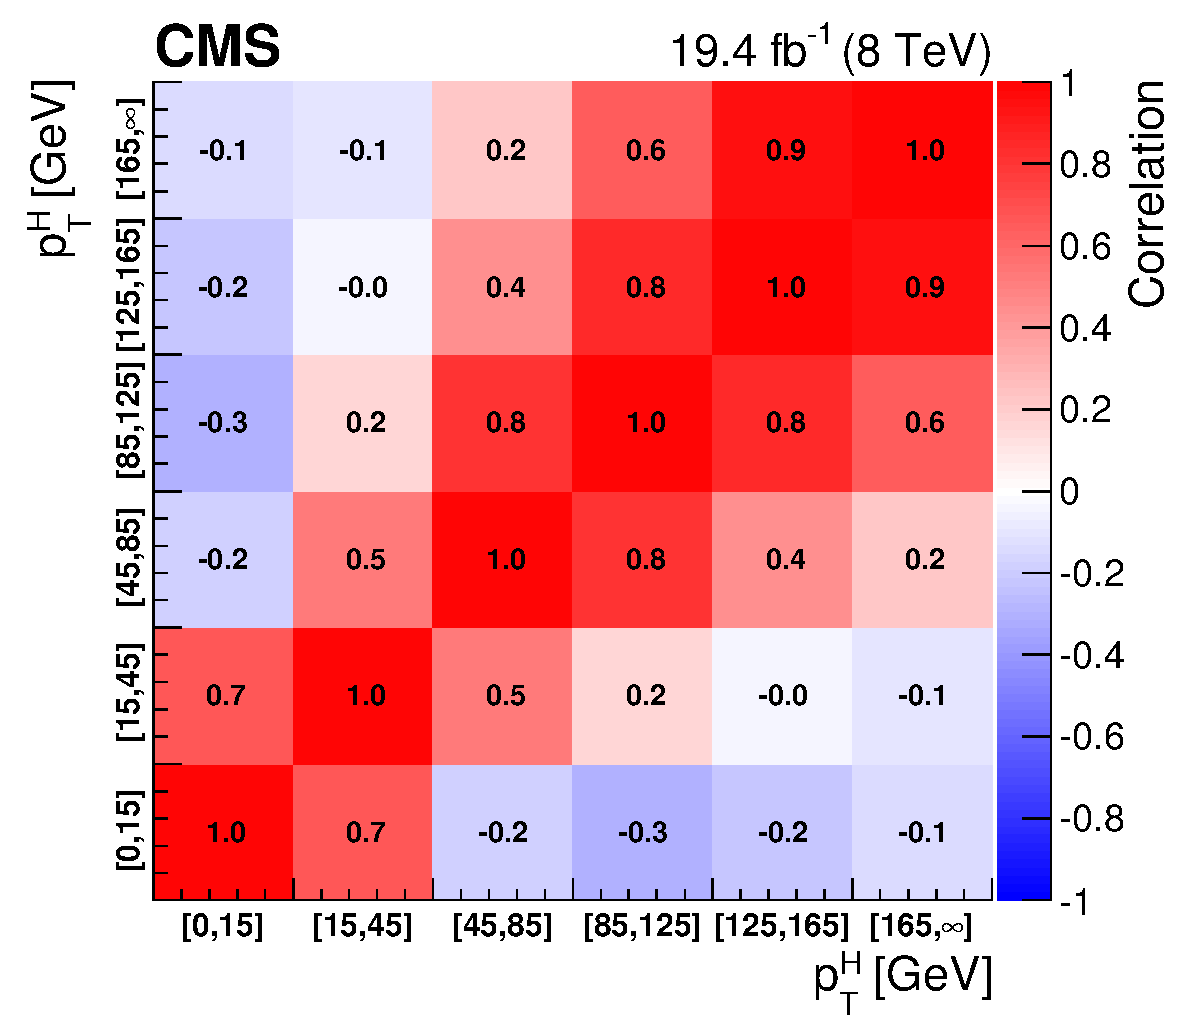
\includegraphics[width=0.6\textwidth]{images/unblinding/covMatrix.pdf}
\caption{Correlation matrix among the \pth~ bins of the differential spectrum.}\label{fig:cov_matrix}
\end{figure}

To measure the inclusive cross section in the fiducial phase space, the differential measured spectrum is integrated over \pth. In order to compute the contributions of the bin uncertainties of the differential spectrum to the inclusive uncertainty,  error propagation is performed taking into account the covariance matrix of the six signal strengths. For the extrapolation of this result to the fiducial phase space, the unfolding procedure is not needed, and the inclusive measurement has only to be corrected for the fiducial phase space selection efficiency $\epsilon_{\rm{fid}}$. Dividing the measured number of events by the integrated luminosity and correcting for the overall selection efficiency, which is estimated in simulation to be $\epsilon_{\rm{fid}} = 36.2 \%$, the inclusive fiducial $\sigma \times B$, $\sigma_{\mathrm{fid}}$, is computed to be:

\begin{equation}
\sigma_{\mathrm{fid}} = 39\pm 8~(\mathrm{stat}) \pm 9~(\mathrm{syst})~\mathrm{fb} \quad ,
\end{equation} 

in agreement within the uncertainties with the theoretical estimate of $48 \pm 8 ~\mathrm{fb}$, computed integrating the spectrum obtained with the \textsc{Powheg V2} program for the ggH process and including the XH contribution.
